\documentclass[10pt,a4paper,oneside]{scrartcl}

% Linking.
\usepackage{url}
\usepackage[unicode=true,colorlinks=false, pdfborder={0 0 0}]{hyperref}

% Language.
\usepackage[english]{babel}
\usepackage{csquotes}

% Bib Latex.
\usepackage[style=numeric,backend=bibtex]{biblatex}
\addbibresource{bibliography.bib}

% Better use of margins.
\usepackage[hmargin=2cm,vmargin=3cm]{geometry}

% Improves spacing for letters and numbers.
\usepackage{microtype}

% Fancy enumeration.
\usepackage{enumerate}

% Algorithms.
\usepackage{algorithm}
\usepackage[noend]{algpseudocode}

% Math stuff.
\usepackage[fleqn]{amsmath}
\usepackage{amssymb}
\usepackage{amsthm}
\usepackage{times}

\newtheorem{definition}{Definition}

% Allows the use of \includegraphics{...}.
\usepackage{graphicx}
\usepackage[center]{caption}
\usepackage{subcaption}

% Better tables.
\usepackage{tabularx}

% Uber table editor: http://truben.no/latex/table/

\begin{document}

%%%%%%%%%%%%%%%%%%%%%%%%%%%%%%%%%%%%%%%%%%%%%%%%%%%%%%%%%%%%%%%%%%%%%%%%%%%%%%%
% TTITLEPAGE
%%%%%%%%%%%%%%%%%%%%%%%%%%%%%%%%%%%%%%%%%%%%%%%%%%%%%%%%%%%%%%%%%%%%%%%%%%%%%%%
\title{Kung Fu Nao}
\subtitle{Human-Robot Interaction (MKI50)}

\author{ Bas Bootsma (0719080) \and Roland Meertens (3009653)}

\date{\today}

\maketitle

%%%%%%%%%%%%%%%%%%%%%%%%%%%%%%%%%%%%%%%%%%%%%%%%%%%%%%%%%%%%%%%%%%%%%%%%%%%%%%%
% INTRODUCTION
%%%%%%%%%%%%%%%%%%%%%%%%%%%%%%%%%%%%%%%%%%%%%%%%%%%%%%%%%%%%%%%%%%%%%%%%%%%%%%%
\section{Introduction}
Introducing the reader to the topic of learning from robots. 

The topic learning from demonstration is a topic that has seen a huge growth in the last few years.
This topic always consists of teaching a robot how to perform a task via demonstration by a human.  
A new topic is that of learning a human how to perform a task from demonstration by a robot. 

In this report an overview will be given of a robot capable of learning a human how to perform certain ``karate'' movements from demonstration by a robot. 
In this system a robot is able to perform a motion, teach the human how to perform this motion, assess the performance of the human and give extra information on the motions that are performed the worst by the user. 

During our program the user is able to learn three motions: 
\begin{enumerate}
  \item Left hand punch
  \item Defensive block
  \item Right hand punch
\end{enumerate}
The left hand punch and the right hand punch both are simple forward motions of the respective arm. 
The defensive block is a slightly modified version of the ``Gedan barai'' motion used in Karate. 
How this motion should be performed is visible in figure \ref{fig:gedanBarai}. 

\begin{figure}[h!]
	\caption{An instruction on how to perform the Gedan barai}
	\centering
	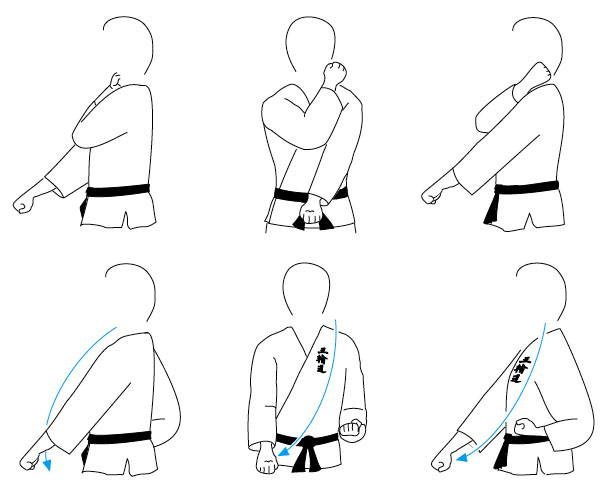
\includegraphics[width=0.5\textwidth]{images/gedanBarai}
	\label{fig:gedanBarai}
\end{figure}

%%%%%%%%%%%%%%%%%%%%%%%%%%%%%%%%%%%%%%%%%%%%%%%%%%%%%%%%%%%%%%%%%%%%%%%%%%%%%%%
% Hardware and Software
%%%%%%%%%%%%%%%%%%%%%%%%%%%%%%%%%%%%%%%%%%%%%%%%%%%%%%%%%%%%%%%%%%%%%%%%%%%%%%%
\section{Hardware and Software}

%%%%%%%%%%%%%%%%%%%%%%%%%%%%%%%%%%%%%%%%%%%%%%%%%%%%%%%%%%%%%%%%%%%%%%%%%%%%%%%
\subsection{Hardware}
In order to build this system the following components were used:
\begin{itemize}
  \item Laptop
  \item Nao robot
  \item Microsoft Kinect
  \item Wireless router
\end{itemize}

The Microsoft Kinect is connected to the laptop using an USB cable and is used to capture the body model of the user. 

The Nao robot is controlled with a wireless connection using the wireless router. 

%%%%%%%%%%%%%%%%%%%%%%%%%%%%%%%%%%%%%%%%%%%%%%%%%%%%%%%%%%%%%%%%%%%%%%%%%%%%%%%
\subsection{Software}
In order to program this system the following software has been used:
\begin{itemize}
  \item Microsoft visual studio 2012
  \item Microsoft Kinect SDK
  \item Choregraph
\end{itemize}


%%%%%%%%%%%%%%%%%%%%%%%%%%%%%%%%%%%%%%%%%%%%%%%%%%%%%%%%%%%%%%%%%%%%%%%%%%%%%%%
% System
%%%%%%%%%%%%%%%%%%%%%%%%%%%%%%%%%%%%%%%%%%%%%%%%%%%%%%%%%%%%%%%%%%%%%%%%%%%%%%%
\section{System}
Discuss the system from an AI point of view.

%%%%%%%%%%%%%%%%%%%%%%%%%%%%%%%%%%%%%%%%%%%%%%%%%%%%%%%%%%%%%%%%%%%%%%%%%%%%%%%
\subsection{Perception}
A way to detect the user and the body model. Do not mention the Kinect.

%%%%%%%%%%%%%%%%%%%%%%%%%%%%%%%%%%%%%%%%%%%%%%%%%%%%%%%%%%%%%%%%%%%%%%%%%%%%%%%
\subsection{Communication}
Gestures + speech...

%%%%%%%%%%%%%%%%%%%%%%%%%%%%%%%%%%%%%%%%%%%%%%%%%%%%%%%%%%%%%%%%%%%%%%%%%%%%%%%
\subsection{World Model}



%%%%%%%%%%%%%%%%%%%%%%%%%%%%%%%%%%%%%%%%%%%%%%%%%%%%%%%%%%%%%%%%%%%%%%%%%%%%%%%
% Individual Components
%%%%%%%%%%%%%%%%%%%%%%%%%%%%%%%%%%%%%%%%%%%%%%%%%%%%%%%%%%%%%%%%%%%%%%%%%%%%%%%
\section{Individual Components}

\subsection{Perception}
Skeleton tracking + dynamic time warping

%%%%%%%%%%%%%%%%%%%%%%%%%%%%%%%%%%%%%%%%%%%%%%%%%%%%%%%%%%%%%%%%%%%%%%%%%%%%%%%
\subsection{Communication}
Note here that we both use speech and gestures. 
Note that we use both beat gestures(gestures without semantic content) as well as metaphoric gestures (gestures indication thinking as well as gestures indication). 

The metaphoric gestures are:
\begin{itemize}
  \item Thinking
  \item Flexing of the muscles
  \item Bowing
\end{itemize}

For speech a word-spotting algorithm is used.
This word-spotting algorithm uses a many-to-one mapping which maps several possible word onto one word that is returned to the system. 
This way the user can use several possible words to confirm a question of the robot. 
The mappings consist of: 
\begin{table}
  \begin{tabular}{ll}
    Keyword & Possible words           \\
    YES     & yes, sure, ETC.          \\
    NO      & no, nope, ETC.           \\
    LEFT    & left, left hand, ETC.    \\
    RIGHT   & right, right hand, ETC.  \\
  \end{tabular}
\end{table}

During the program Naomi will ask the user for input several times. 
Some of the questions are used to keep the user active during the program and are just meant to give the user extra interaction with the robot. 
An example of this question is: ``Have you practiced Robot Karate before?'' after which the robot either will say that it will be an easy lesson or asks the user to give extra attention to the gestures. 
Other questions are used by the robot to give specific feedback.
An example of this question is asked during the performance of the defensive block: ``Are you having more trouble with your left or with your right arm'', after based on the input of the user the robot will explain only one arm of the defensive block. 

%%%%%%%%%%%%%%%%%%%%%%%%%%%%%%%%%%%%%%%%%%%%%%%%%%%%%%%%%%%%%%%%%%%%%%%%%%%%%%%
\subsection{World Model}

%%%%%%%%%%%%%%%%%%%%%%%%%%%%%%%%%%%%%%%%%%%%%%%%%%%%%%%%%%%%%%%%%%%%%%%%%%%%%%%
\subsection{Graphical User Interface}



%%%%%%%%%%%%%%%%%%%%%%%%%%%%%%%%%%%%%%%%%%%%%%%%%%%%%%%%%%%%%%%%%%%%%%%%%%%%%%%
% Interaction
%%%%%%%%%%%%%%%%%%%%%%%%%%%%%%%%%%%%%%%%%%%%%%%%%%%%%%%%%%%%%%%%%%%%%%%%%%%%%%%
\section{Interaction Patterns}


\begin{figure}[h!]
	\caption{State diagram showing in what order the behaviours of the robot are performed}
	\centering
	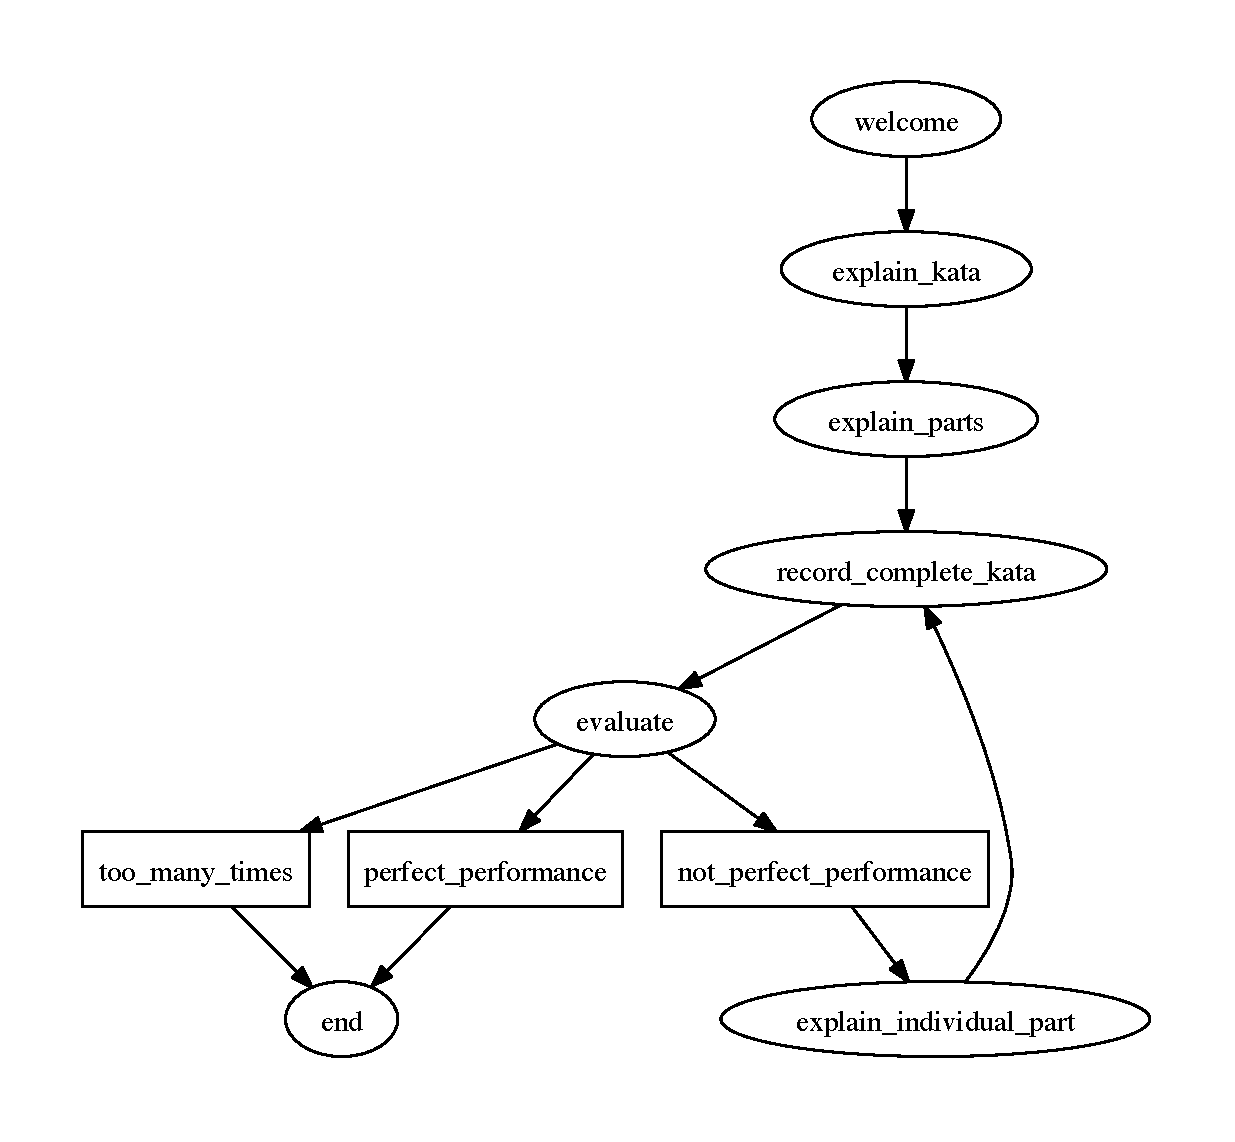
\includegraphics[width=0.5\textwidth]{images/stateDiagram}
	\label{fig:overviewTotalSystem}
\end{figure}

%%%%%%%%%%%%%%%%%%%%%%%%%%%%%%%%%%%%%%%%%%%%%%%%%%%%%%%%%%%%%%%%%%%%%%%%%%%%%%%
% Conclusion
%%%%%%%%%%%%%%%%%%%%%%%%%%%%%%%%%%%%%%%%%%%%%%%%%%%%%%%%%%%%%%%%%%%%%%%%%%%%%%%
\section{Conclusion}



%%%%%%%%%%%%%%%%%%%%%%%%%%%%%%%%%%%%%%%%%%%%%%%%%%%%%%%%%%%%%%%%%%%%%%%%%%%%%%%
% BIBLIOGRAPHY
%%%%%%%%%%%%%%%%%%%%%%%%%%%%%%%%%%%%%%%%%%%%%%%%%%%%%%%%%%%%%%%%%%%%%%%%%%%%%%%
\printbibliography

\end{document}
